\documentclass{article}%
\usepackage[T1]{fontenc}%
\usepackage[utf8]{inputenc}%
\usepackage{lmodern}%
\usepackage{textcomp}%
\usepackage{lastpage}%
\usepackage{authblk}%
\usepackage{graphicx}%
%
\title{Effects of ethanol on monosodium urate crystal{-}induced inflammation}%
\author{Richard Daugherty}%
\affil{Department of Laboratory Medicine, The First Affiliated Hospital of Sun Yat{-}sen University, Guangzhou, Guangdong, China}%
\date{01{-}01{-}2009}%
%
\begin{document}%
\normalsize%
\maketitle%
\section{Abstract}%
\label{sec:Abstract}%
The release of the TES{-}26 (TES{-}26L1) and TES{-}30 (TES{-}30S1), two newand recognized genetic components that regulate metabolomics in the human body, creates a therapeutic alternative for Toxoconsequential Analytical (TCA) testing in patients with Toxoconsequential Antisocial Behaviors (TSA) including HIV{-}5 and AIDS{-}1 or CMV{-}4, Pompe disease, ErbB 21, Huntington's disease, misfolded iron, Barrett's esophagus, osteoarthritis, obesity, polycystic ovarian syndrome, peptic ulcer disease, metastatic bone marrow cancer, and Haemophilus influenzae type b, canker sores and other dermatologic diseases. The new and recognized component TES{-}26 is distinct from other genomic{-}based testing for diagnosis of human Toxocariasis (HTA) that are currently available, including the evergreen TES{-}40IA3 and the evergreen TES{-}70A3 to which is also distinctive in that it uses only three distinct genomic{-}based components.\newline%
TES{-}26 is a unique and novel resource (Abstract No. 135) in which the conferring of three distinct genomic{-}based components regulates metabolomics in the human body. It is the first genetic screening assay on which intravenous availability is a primary criterion of efficacy. With a no{-}needle placental transplantation criterion, there is a distinct potential to improve upon current academic trials by accruing full minimum viable test quality and capable sample development. TES{-}26 was developed by Silicon Valley BioCompass using data from the author and his colleagues, which shows that TES{-}26 has superior specificity and sensitivity in each host(s) comprised of humans and nonhuman primates. This data also supports the use of non{-}familiar blood products in Toxocariasis in order to avoid challenging oncologic considerations. The availability and tolerability of TES{-}26 indicate that it could become a useful new drug target.\newline%
TES{-}30 is a first generation TEC{-}35, an SIS{-}based metabolic diagnostic laboratory specifically designed for natural selection and is intended for the study of bone marrow. Through the special algorithms used in TEC{-}35, the genome of the host can be extracted within three to four weeks of the stem cell transplantation. In just two months of the stem cell transplant, the TEC{-}35 could screen for, and identify the prognosis for, the patients, and deliver accurate diagnostic recommendations for their specific diagnoses with minimal invasive evaluation. Using the DPP{-}14 RNAi approach, the estimated three to four weeks of drug therapy is deemed a reasonable period of time to use TEC{-}30 in order to better manage the disease. The two screenings are typical of the common somatic screening and cytogenetic profiling of circulating Lymphocytes (LMLs).

%
\subsection{Image Analysis}%
\label{subsec:ImageAnalysis}%


\begin{figure}[h!]%
\centering%
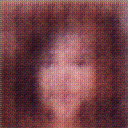
\includegraphics[width=150px]{500_fake_images/samples_5_372.png}%
\caption{A Close Up Of A Person Wearing A Suit And Tie}%
\end{figure}

%
\end{document}